\documentclass[12pt]{thesis}

% The LaTeX default font is Computer Modern Roman for text and
% math. We will switch to times roman, because that is preferred by
% the Graduate school.  However, you can comment the times fonts and
% uncomment one (or more) of the others to choose a different font set.
\usepackage{mathptmx}   % Times New Roman with matching math fonts
% \usepackage{newcent}  % new century schoolbook font
% \usepackage{bookman}  % bookman font
% \usepackage{fourier}  % Utopia (text) and Fourier (math) font


\usepackage{graphicx}
\usepackage{rotating}
\usepackage{makeidx}
\usepackage{subfig}
\usepackage{indentfirst}

%% Uncomment the following two lines and comment out the third one
%% if you want to use the Chicago Manual based bibliography.
% \usepackage{thesiscitations}
% \bibliographystyle{thesis}
\bibliographystyle{ieeetr}

%% Change ieeetr in the previous line to any bibliography style you
%% like

%% Uncomment next line if you want chapter titles centered (not
%% approved by SDSMT graduate school)
% \centertitles

%% Uncomment next line to print a double-spaced draft version
% \dsdraft

%% Uncomment next line to print a single-spaced draft version
% \ssdraft

%% Uncomment next line if you are using makeindex to create an index
% \makeindex

\doctype{thesis}
\title{A Compative Study of Gnus and Gnats: The Most Important Paper Ever Written}
\author{Harvey Finklebaum}
\degree{Doctor of Philosophy in Zoology}
\defensedate{April 4, 2013}
\gradyear{2013}
\department{Zoology}

% The following commands add a signature line for each person who needs
% to sign the thesis/dissertation
\signatureline{Major Professor --- Dimm Whitt, Ph.D., Department of
  Zoology}

\signatureline{Graduate Division Representative --- E.\ Nigma, Ph.D.,
  Department of Philosophy}

\signatureline{Committee Member --- Chip Munk, Ph.D., Department of
  Zoology}

\signatureline{Committee Member --- Gail Force, Ph.D., Department of
  Meteorology }

\signatureline{Head of the Zoology Department --- Earl E. Byrd, Ph.D.}

\signatureline{Dean of Graduate Education --- Raney Daze}

\begin{document}

\maketitle

%% Comment the next line to remove the copyright notice.  Read the
%% section on copyright in the Thesis and Dissertation Writing
%% Instructions.
\makecopyright % copyright must go BEFORE \preliminaries


\preliminaries


\begin{abstract}
I present a fascinating and
thought provoking study, comparing gnus and gnats.
The results of the study show conclusively that there
is no resemblance between the two, whatsoever.
\end{abstract}

%% Uncomment the following if you want acknowledgements
\begin{acknowledgments}
  I would like to thank my advisor, Dr.\ Dimm Whitt, for
  all of the support he has given me. It really was not much,
  but he did at least stop yelling at me.
\end{acknowledgments}

\tableofcontents

\listoftables

\listoffigures

%% Uncomment following lines if you want a list of symbols
%% \gltitle{List of Symbols}
%% \begin{genericlist}
%% \begin{tabular}{ll}
%%   $\mathcal{G}_t$ & Gnat\\
%%   $\mathcal{G}_u$ & Gnu
%% \end{tabular}
%% \end{genericlist}

%% Uncomment following lines if you want a list of keywords
%% \gltitle{List of Keywords}
%% \begin{genericlist}
%% \noindent Gnat, Gnu
%% \end{genericlist}

%% Uncomment following lines if you want a dedication
% \begin{dedication}
% In loving memory of 
% my grandmother.
% \end{dedication}

%% Uncomment following lines if you want a preface
% \begin{preface}
% Before we begin, just let me say one thing.
% Gnat and gnu are both begin with ``gn,'' and
% the purpose of this work was to see if there
% are any other resemblances.
% This thesis has taken 45 years of work, and
% I don't have much time left in this world, but it
% has been worth it.  When the time comes,
% I would like to die as my grandmother did, peacefully in
% her sleep, not screaming like the passengers in her car.
% \end{preface}


\body


\chapter{Introduction}
\section{Reinforcement Learning}
Reinforcement Learning (RL) is a subset of Machine Learning where an agent takes actions within an environment to maximize some environmental reward. This is a wide field that includes robotic arm manipulation, video game playing, path-planning, and many other areas.

In RL, the environment is the problem space. In the case of an assembly line, the environment would contain the robot arm, the conveyor belt, the items on the belt, and other related aspects. Every time-step, the environment updates. Items move along the belt, the robot arm shifts, etc.

The agent is the part of the program that learns and adapts to its environment. In the same case of the assembly line, the agent is the robotic arm. Every time-step, the agent receives its current state ‘s’ from the environment. In our current example, the state can be represented as the angle and rotation of the joints in the arm as well as whether the arm’s gripper is open or closed. Once the agent has received its current state from the environment, it decides what action ‘a’ to take from the set of all possible actions ‘A’. In our example, this could be telling the arm’s third motor to move to a specific angle and rotation or activating/releasing the gripper.

When an agent takes an action, it gets feedback from the environment in the form of a reward. This reward is a measure of how good the agent’s choice was. For example, if the robot arm successfully created a product, it could get a reward based on the product’s quality. On the other hand, if the robot arm had smashed into a wall, the agent could get a negative reward known as a punishment. The agent can use these rewards to adjust its behavior to maximize the total reward it can get.

Taken together, the system works as follows. The environment gives a state ‘s’ to the agent, who uses that state to determine the action ‘a’ it takes. The environment then gives a reward ‘r’ to the agent (usually with the next state s’) which it uses to learn whether it should take that action again next time it is in that state.

By repeating this process over many time-steps, the agent will eventually learn the best actions to take in order to maximize the total reward.

\subsection{Intrinsic reward systems}
Although the above explanation of Reinforcement Learning works in many cases, it struggles to solve problems where environmental rewards are infrequent or spread sparsely throughout the environment.

One simple example of this is the case of a robot stuck in a maze. Since the robot only gets rewarded when it successfully exits the maze, the robot has no feedback until it succeeds for the first time. For any maze of significantly large size, it practically impossible for the robot to randomly stumble upon the correct solution. As such, a robot depending on external (environmental) reward to learn is not sufficient to solve this problem.

Intrinsic rewards are one method to allow agents to learn without the presence of environmental rewards. By letting the agent reward itself when it learns about the environment, the agent can learn to maximize its exploration of its environment. Once the agent has found external rewards, more traditional learning utilizing external rewards may be achieved.

One simplistic intrinsic reward system is to reward the agent whenever it finds a state it has never encountered before. This encourages the agent to seek out new states, allowing it to explore its environment more efficiently. This method has problems as discussed later but is significantly better than random exploration. (Taking random actions)

\section{Noisy TV Problem}
The Noisy TV Problem is a particularly difficult scenario when using intrinsic reward systems in Reinforcement Learning. The problem is as follows: What if within the environment there was a TV with a remote. Whenever the agent was in front of the TV it could press the remote to switch the TV to a random channel.

Many intrinsic reward systems fall prey to this scenario. For example, the intrinsic reward system above that rewards finding new states would consider the TV to be extremely valuable since all it takes is a single action to find a new state! This is significantly better than exploring around over multiple time-steps to find new areas not seen before. What makes this problem particularly difficult is that the agent cannot tell the difference between moving from state to state around the problem space and pressing the button to flip the channel. Both of these things are taking an action based on a given state.

Other intrinsic reward systems such as count-based methods, probabilistic methods, and even memory methods fall prey to this problem.

\section{Predicted Information Gain (PIG)}
PIG is an algorithm that uses information theory to maximize exploration of the environment. PIG functions by predicting how much information about the environment the agent will learn for each action it could take, then taking the action with the most information gain. This means that PIG focuses on creating the best model of the world it can, rather than maximizing the reward obtained from the environment.

\subsection{KL-Divergence}
To determine the amount of information that can be gained from entering a new state, PIG uses the Kullback-Leibler (KL) divergence. The KL-divergence determines the similarity of two probability distributions. In our case, it is the average amount of information that would be lost if we represented one probability distribution with code optimized for the other distribution.

The equation for the KL-divergence is as follows:
\[D_{KL} (\Theta_{as\cdot} || \hat{\Theta}_{as\cdot}) := \sum_{s' = 1}^{ N} \Theta_{ass'} \log_{2}(\frac{\Theta_{ass'}}{\hat{\Theta}_{ass'}})   \]

Where $\Theta$ is the true probabilities of state transition from state $s$ to state $s'$ by taking action $a$, $\hat{\Theta}$ is the agent's estimation of $\Theta$ based on its experiences, and $N$ is the number of valid possible state transitions from $s$ to $s'$.

\subsection{Information Gain/Missing Information}
PIG calculates the amount of information that would be gained by taking a specific action by averaging the amount of information that each state transition would give multiplied by the chance of achieving that state transition. The equation is as follows:

\[ PIG(a,s) := E_{s^{*},\Theta|\vec{d}} [I_{G}(a,s,s^{*})] = \sum_{s*} \hat{\Theta}_{ass^{*}}D_{KL}(\hat{\Theta}_{as\cdot}^{a,s \rightarrow s^{*}} || \hat{\Theta}_{as\cdot}) \]

Where $s^{*}$ is a valid resulting state due to taking action $a$ in state $s$ and $\hat{\Theta}_{as\cdot}^{a,s \rightarrow s^{*}}$ is the updated model of $\hat{\Theta}_{as\cdot}$ if a transition from $s$ to $s^{*}$ was observed.

Intuitively, $D_{KL}(\hat{\Theta}_{as\cdot}^{a,s \rightarrow s^{*}} || \hat{\Theta}_{as\cdot})$ is a measure of how different our new model would be compared to our current model if we successfully transitioned from $s$ to $s^{*}$.

Since the above equation is fully dependent on our internal model rather than the true model of the environment, it is updated whenever new data is learned and can be applied even when the agent is unaware of the true nature of the environment (As is the case in most real-world problems). In fact, the above equation can even be applied when the agent has no understanding of the problem space whatsoever but merely has a method of observing and interacting with its environment.

\section{Thesis Statement}
The PIG algorithm still falls prey to the Noisy TV problem. When in the Noisy TV state, the PIG algorithm will predict that there is a lot of information to be gained by using the controller. This is because pressing the controller takes the agent to a state significantly different from the state it is currently in, making the KL-divergence between the two states large. Even though the PIG algorithm takes the weighted average of the information gain based on how likely it is to get to that state, it will still consider pressing the controller to be valuable because every state it could reach through the Noisy TV has a high KL-divergence.

The largest cause of this problem is that there is no confirmation that information has actually been learned. The PIG algorithm predicts future information gain based on it’s current data, but it never confirms that its prediction was correct.

As such, I suggest changing the PIG algorithm to make it more robust to the Noisy TV problem. After each time-step, the new algorithm will re-calculate the Predicted Information Gain with the updated models from including the previous step. It will then compare the prediction from before with the new prediction. If information was actually learned the new prediction will be lower then the previous prediction as the total amount of information left to be learned has decreased. This decrease in unlearned information will then be normalized and used as an intrinsic reward.

When this new method, PIG++, encounters the Noisy TV problem it will quickly realize that although the TV looks like it will provide a large amount of information, it actually provides very little that is useful.

\chapter{Previous Work}


There has been a lot of previous work that is not at all like my work.
For example,
% The following if-then-else allows us to get good results with
% any bibliography/citation style.
\ifthesiscitations
\citeN{Kringle} % if we are using the thesiscitations style
\else
Kringle~\cite{Kringle} % if we are using a more primitive citation style
\fi
showed that apples and goats have almost
nothing in common, other than both being red.  The major problem with
Kringle's study is that he used a goat that had been spray painted
red, and his apple was a golden delicious variety.  Criticism of
Kringle's methods has been harsh, and so far, no one has been able to
replicate his results.

Several researchers have compared trout to
eagles~\cite{Simmons,Sheppard}.  The consensus that has emerged is
that they are quite different, and only an idiot would try to eat an
eagle~\cite{Idiot}.

\chapter{Methods}
In this chapter, I will present the methods for my comparison, and
fill in with a lot of gibberish.  For instance, I will say things like
``Gnats and Gnus come in twos'' in order to fill space and make my
thesis seem longer than it really is.  This is a tactic used by some
people to hide the fact that their research is worthless.  The idea is
that if the thesis is long enough and boring enough, the thesis
comittee members will go to sleep every time they try to read it.

Another thing that I may do is to use very long words, such as
onomatopoeia, for no apparent reason.  By employing voluminous
instances of obfuscatory and expansive vocables, the lack of
quintessence of this monograph can be adumbrated from all but
the most erudite, didactic, and scholarly bibliophiles.


\chapter{Results}
My research had fabulous results. I will now tell you about
the results, because they are the best!  You are not going
to believe how good my results are.

\section{Visual comparison}
%\index{comparison!visual}

\begin{table}
\caption{Results of visual comparison studies.}
\begin{center}
  \begin{tabular}{|c|c|}
    \hline
    \bf Categories & \bf Percent Correct\\
    \hline
    \hline
    insect/mammal & 76\\
    \hline
    gnat/gnu & 69\\
    \hline
  \end{tabular}
\end{center}
\label{table:comp1}
\end{table}

The first test that I performed was a visual comparison of gnats and
gnus.  First, I went on the internet and downloaded several thousand
pictures of gnats, and one picture of a gnu.  Then, I had two
volunteers compare them and categorize them as insect
%\index{insect}
or mammal.
%\index{mammal}
Next, I selected another group of volunteers and
had them classify the photographs as either gnat or gnu.


\begin{sidewaysfigure}
\begin{center}
\subfloat{\resizebox{0.45\textheight}{!}{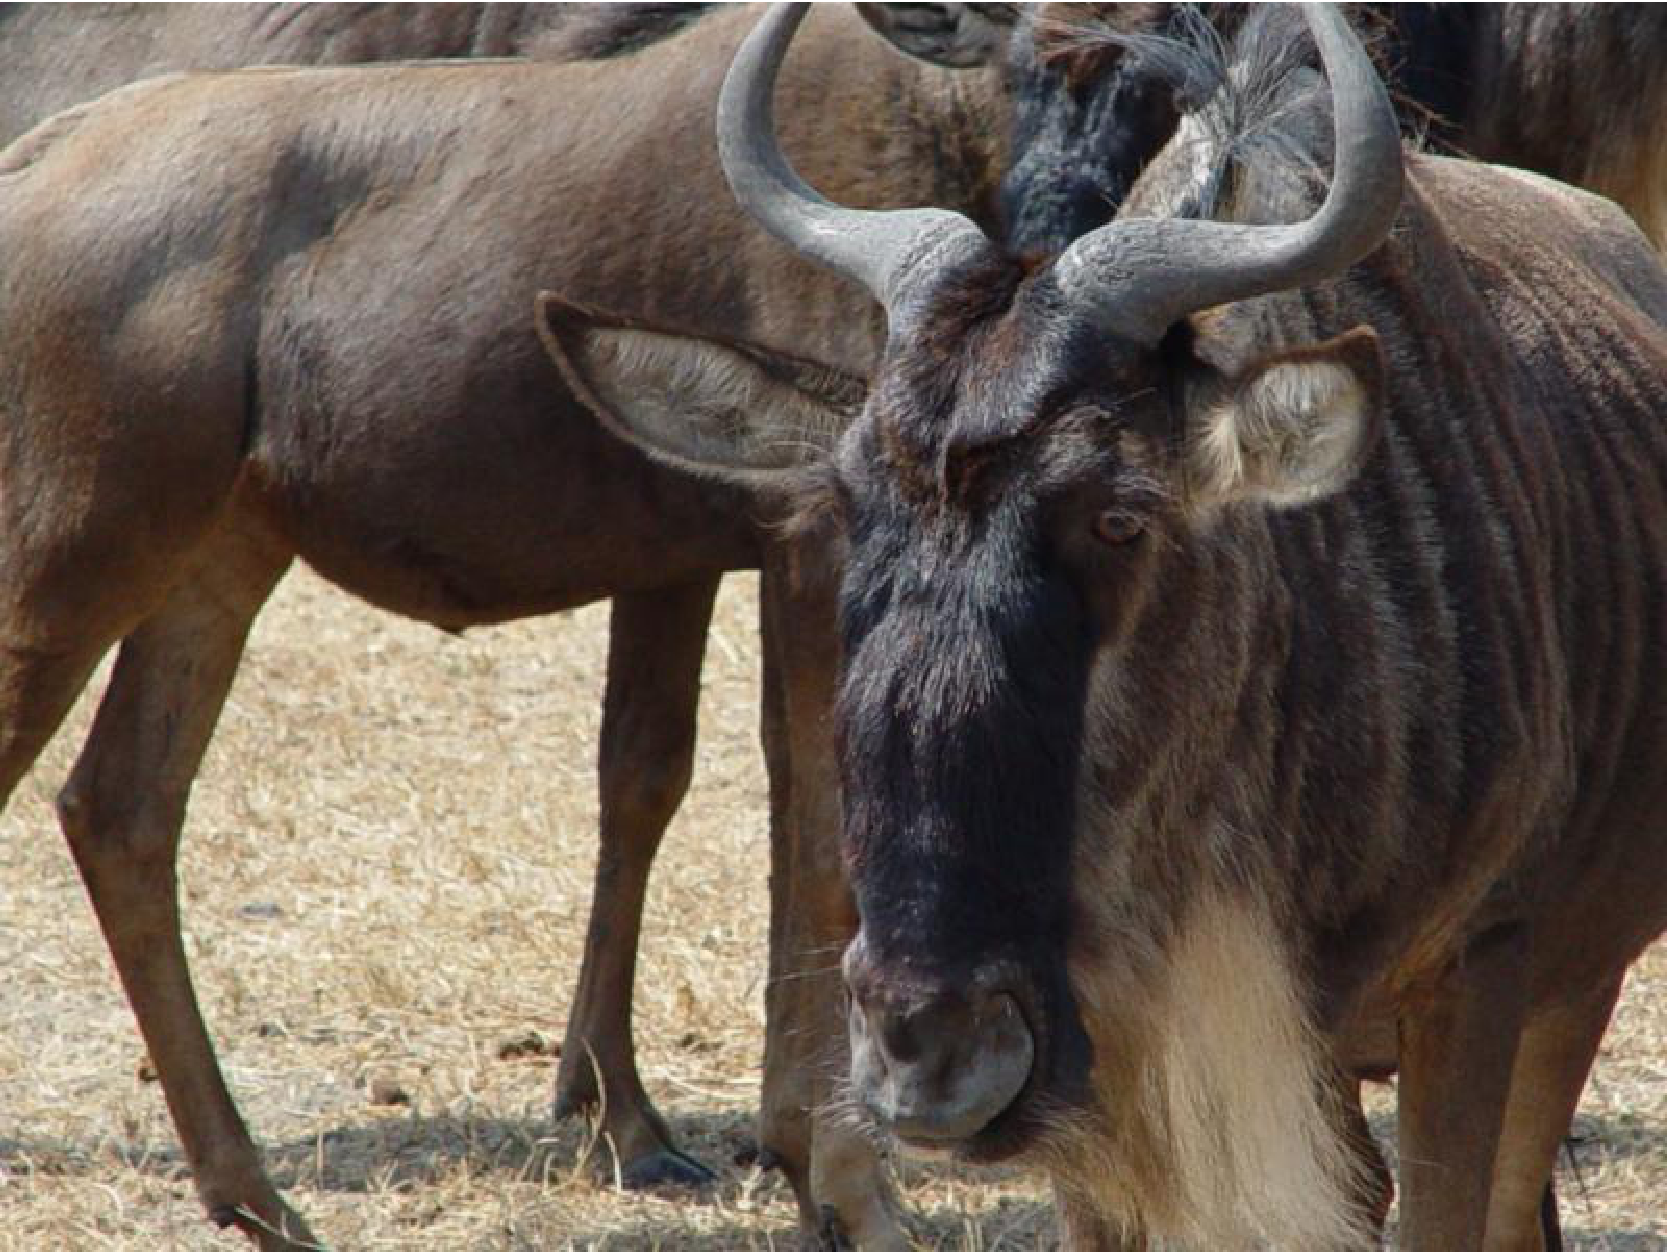
\includegraphics{images/gnu.pdf}}}
\subfloat{\resizebox{0.45\textheight}{!}{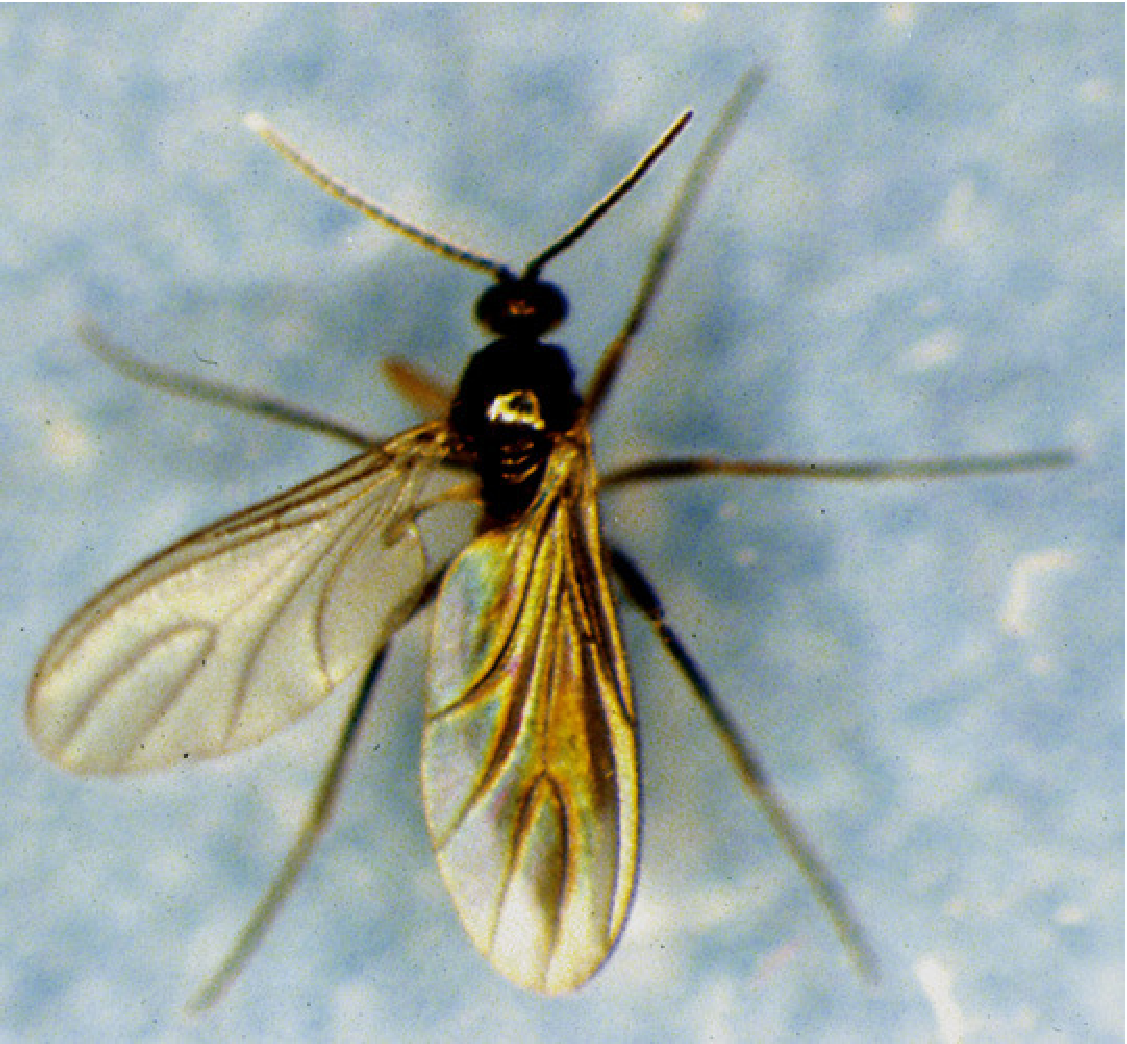
\includegraphics{images/gnat.pdf}}}
\end{center}
\caption{Photographs of a gnu (left) and a gnat (right).}
\label{figure:photos}
\end{sidewaysfigure}

The results of this comparison are shown in Table~\ref{table:comp1}.
As can be seen, both volunteers (myself and my advisor) were able to
correctly classify most of the photographs.  As a result, we gave each
other little gold stars.
For those who are interested, Figure~\ref{figure:photos} shows the gnu
photograph and one of the gnat photographs.

\section{Comparison by Size}
\index{comparison!size} As can be seen from
Figure~\ref{figure:photos}, photographs of gnats are slightly larger
than photographs of gnus.  This leads us to believe that
statistically, gnats are slightly larger than gnus.  Mathematically,
we express this as follows:
\begin{equation}
S(\mathcal{G}_t) > S(\mathcal{G}_u) \forall
\mathcal{G}_t,\mathcal{G}_u,
\end{equation}
where $\mathcal{G}_t$ is a photograph of a gnat and $\mathcal{G}_u$ is
a photograph of a gnu.  The $S()$ function calculates the ``size'' of
the photograph.

\chapter{Conclusions}

Well, there you have it.  My advisor and I were able to tell the
difference between a photograph of a gnat and a gnu most of the time.
Also, gnats are larger than gnus, and therefore, they are
significantly different.

In the future, we plan to apply the techniques developed in this
research to answer the age old question of whether dogs and ducks are
the same thing.

\supplementaries


\bibliography{harvey}


\begin{appendices}

\appendix{Appendix A} Well, I really have nothing more to say,
but wanted to have an appendix.

\end{appendices}

%% Uncomment the following lines if you want to create a glossary
% \begin{gloss}
% I don't have a glossary either, but this is what the page would look
% like if I did.
% \end{gloss}


%% uncomment following lines if you want to create a list of abbreviations
% \begin{abbreviations}
% gnu is abbreviated to gnu\\
% gnat is abbreviated to gnat
% \end{abbreviations}

%% uncomment next line if you used makeindex to make an index
%\printindex

\begin{vita}

  
  Format the vita page according to the following graduate school requirements:

A vita page, not over one page in length, is to be included as the
last page of all theses and dissertations deposited in the Devereaux
Library. The vita is to be written in the third person using
professional style and could contain the following information
(although you may wish to omit A and B if concerned about identity
theft):
\begin{enumerate}[label=\Alph*.]
\item Place and date of birth.

\item Place and date of high school graduation.

\item Place and date of college graduation—with degree and major.

\item Place and date of receipt of master’s degree—with major.

\item Vocational and professional experience (not summer jobs)—including dates, nature of position, and school or organization.

\item Military experience, with indication of professional relevance—if any.

\item Scholarly publications, exhibits of creative work, membership in professional organizations and honorary societies.
\end{enumerate}
  

\end{vita}



\end{document}
